\section{Background: quantization and quantification} \label{sec:background}

\begin{figure}
    \centering
    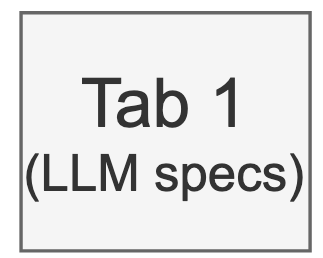
\includegraphics[width=0.75\linewidth]{reportTemplate/figures/f2.png}
    \caption{Caption}
    \label{fig:background}
\end{figure}

In this section, we present background on LLM quantisation and a high-level overview of this compression technique in~\Cref{fig:background}. Then, we present background on metrics and techniques used to quantify accuracy, energy consumption, and CO2 emissions. 

Quantization is \textit{"the division of a quantity into a discrete number of small parts, often assumed to be integral multiples of a common quantify``}~\cite{DBLP:journals/corr/abs-2411-0253}. In LLMs, quantization is a compression technique that reduces the precision of model parameters from standard representation (e.g., 32-bit floating point) to lower-bit representation (e.g., 8-bit integers). Post-training quantization (PTQ) is preferred, primarily due to
the extensive computational demands associated with fine-tuning for Quantization Aware Training~\cite{zhang2023dual, DBLP:conf/icml/NagelABLB20, DBLP:journals/corr/abs-2006-10518}. In this work, we adopt PTQ as our compression method, thus adhering to the state-of-the-art in the community.

We use metrics for quantifying operational-level metrics. We adhere to international system measurements and community standards and quantify energy consumption in kilowatt-hour (kWh) and CO2 emissions in grams of CO2. To derive CO2 emission from energy consumption, we follow the vetted approach proposed by Niewenhuis et al. in Footprinter~\cite{DBLP:conf/wosp/NiewenhuisTIM24}; we present this formula in \Cref{eq:CO2-emissions}, where $C_e$ is the total amount of CO2 emissions, $C_i$ is the carbon intensity, and $E$ is the total energy consumption.

\vspace*{-0.7cm}
\begin{align}
    C_{e} = C_{i} \times E
    \label{eq:CO2-emissions}
\end{align}
\vspace*{-0.6cm}

To quantify accuracy, we will be using Evaluate  library for python, which is a tool to apply many different and well-accepted accuracy metrics, such as BLEU, which is often used to evaluate machine-translations or F1 score, which is the harmonic mean of precision and recall. Since different metrics are best suited to different uses of the LLM, we decided that using ‘Evaluate’s metric collection interface would be the most efficient option. 
	
For the metrics, while this is subject to change, we have decided to use BLEU, F1 and BERT-score, and evaluating these various results to not only find which LLM’s are the most accurate, but also in which categories they are most affected by the compression.


